\documentclass{article}

\usepackage{../../uni-notes-eng}

\title{referacik}
\author{dupa chuj \and kurwa szmata}
\date{21.37}

\newcommand{\T}{\rodz{T}}

\begin{document}
\maketitle
\thispagestyle{empty}

\tableofcontents

\subsection{Powtórka tego co było}

{\large\color{def}DYFEOMORFIZM} to funkcja $h:U\to V$ dla otwartych $U,V\subseteq\R^n$ która jest klasy $C^\infty$ i jej odwrotność $h^{-1}:V\to U$ jest również klasy $C^\infty$. {\large\color{def}$k$-WYMIAROWA ROZMAITOŚĆ} to podzbiór $M\subseteq\R^n$ taki, że dla każdego punktu $x\in M$ istnieje otwarty podzbiór $x\ni U\subseteq\R^n$, otwarty podzbiór $V \subseteq\R^n$ oraz dyfeomorfizm $h:U\to V$ taki, że
$$h(U\cap M)=V\cap (\R^k\times\{0\})=\{y\in V\;:\;y^{k+1}=...=y^n=0\}$$
czyli $U\cap M$ jest z dokładnością do dyfeomorfizmy po prostu $\R^k\times\{0\}$.
\medskip

{\large\color{def}UKŁAD WSPÓŁRZĘDNYCH} wg. Spivaka to różnowartościowa funkcja $W\to\R^n$ dla otwartego $W\subseteq\R^k$ taka, że

\point $f(W)=M\cap U$

\point $f'(y)$ ma rangę $k$ (czyli obraz ma wymiar $k$) dla każdego $y\in W$

\point $f^{-1}:f(W)\to W$ jest ciągła.
\medskip

{\large\color{def}TENSORY}
\begin{description}
    \item [$k$-tensor] to funkcja $k$-liniowa $T:V^k\to\R$ dla $V$ - przestrzeni liniowej nad $\R$. Zbiór wszystkich $k$-tensorów oznaczamy $\rodz{T}^k(V)$ i wymagamy, żeby to była przestrzeń liniowa (dodawanie, mnożenie przez skalary ma śmigać)
    \item [Iloczyn tensorowy] dla $S\in\T^j(V)$ oraz $T\in\T^k(V)$ to $S\otimes T\in\T^{j+k}(V)$i definiujemy go: $$(S\otimes T)(v_1,...,v_{k+j})=S(v_1,...,v_j)\cdot T(v_{j+1},...,v_{k+j}),$$ bo przecież $S$ i $T$ to tak naprawdę skalary, więc sprowadza się to do mnożenia skalarów, tylko musimy zmienić dziedzinę żeby śmigało :v
    \item Jeśli $e_1,...,e_d$ jest bazą $V$, a $\phi_1,...,\phi_d$ jest jej bazą dualną, to zbiór wszystkich iloczynów tensorowych $k$ elementów bazy dualnej jest \textbf{bazą przestrzeni $\T^k(V)$}.
    \item Dla odzworowania liniowego $f:V\to W$ definiujemy odwzorowanie liniowe $f^*:\T^k(W)\to\T^k(V)$ jako $$(f^*T)(v_1,...,v_k)=T(f(v_1),...,f(v_k))$$
\end{description}
\medskip

{\large\color{def}TENSORY ALTERNUJĄCE}
\begin{description}
    \item [Tensor alternujący] $\omega$ to taki, że dla dowolnego $\sigma\in S_k$ mamy $$\omega(v_{\sigma(1)},...,v_{\sigma(k)})=(sgn(\sigma))\omega(v_1,...,v_k)$$ Przestrzeń liniową tensorów alternujących oznaczamy $\Omega^k(V)$ (lub$\Lambda^k(V)$, jeżeli jesteśmy Spivakiem)
    \item Przekształcenie $Alt:\T^k(V)\to\Omega^k(V)$ definiowane $Alt(T)(v_1,...,v_k)=\frac1{k!}\sum_{\sigma\in S_k}(sgn(\sigma))T(v_{\sigma(1)},...,v_{\sigma(k)})$ jest liniowe.
    \item [Iloczyn zewnętrzny tensorów alternujących] jest definiowany dla $\omega\in\Omega^k(V)$ i $\eta\in\Omega^j(V)$ jako $$\omega\land\eta={(k+1)!\over k!j!}Alt(\omega\otimes\eta)\in\Omega^{k+j}(V)$$
    \item Zbiór wszystkich $k$-krotnych iloczynów zewnętrznych $\phi_i$ jest \textbf{bazą przestrzeni} $\Omega^k(V)$.
\end{description}

{\large\color{def}POLA}
\begin{description}
    \item[Przestrzeń styczna] w punkcie $p\in\R^d$ jest definiowana jako $$T_p\R^d=\R^d_p:=\{(p,v)\;:\;p,v\R^d\}$$ i określamy na niej działanie $(p,v)+(p,w)=(p, v+w)$ oraz $a(p, v)=(p, av)$.
    \item[Wiązka styczna] w punkcie $p$ to zbiór $\{(p,v)\;:\;p\in\R^d,v\in\R^d\}=\bigcup\limits_{p\in\R^d}T_p\R^d$
    \item[Pole wektorowe] zmienia definicje z $F:\R^d\to\R^d$ zadanego $F(p)=(F_1(p),...,F_d(p))$ na $F:\R^d\to T\R^d$ zadanego wzorem $F(p)=(p,\sum\limits_{i=1}^d F^i(p)e_i)$ dla wektorów bazowych $e_i$. Pola wektorowe można dodawać i mnożyć przez funkcjonał.
    \item To samo możemy zrobić dla $1$-tensorów, czyli funkcjonałów - podmieniamy w definicji wiązki stycznej wektor $v$ na funkcjonał i dostajemy $T^*\R^d\approx\R^d\times\Omega^1(\R^d)$.
\end{description}

\section{Rozmaitości i takie tam}

{\large\color{def}FORMY}
\begin{description}
    \item Mówimy, że funkcja $\overline{\phi}:\R^d\to T^*\R^d$ jest nazywana \textbf{cięciem} $T^*\R^d$, a z kolei $\overline{\omega}:\R^d\to\Omega^k(T\R^d)$ jest \textbf{cięciem $T\R^d$}. Alternatywnie, te funkcje nazywamy odpowiednio \textbf{\color{acc}1-formą i $k$-formą}.   
    \item Mimo, że wszystkie funkcjonały zapisują się jako suma $\overline{\phi_i}(E_j)=\delta_{ij}$ przemnożona przez $a_i(p)$, ale nie jest to baza, bo $a_i$ to funkcjonał a nie skalar
    \item Jeżeli $f:W\to \R^n$ jest układem współrzędnych, a $\omega$ jest $k$-formą na $M$ to $f^*\omega$ jest $k$-formą na $W$.
    \item {\color{def}NOWE OZNACZENIE: $dx^i=\overline{\phi_i}$.}
    \item Dowolną $k$-formę możemy zapisać jako $$\omega=\sum\limits_{i_1<...<i_k}\omega_{i_1...i_k}dx^{i_1}\land ...\land dx^{i_k}$$ gdzie $\omega_{i_k}$ to funkcje na $\R^d$ a $\omega$ powinna mieć kreseczkę, ale używamy notacji ze Spivaka :3 Jeśli te funkcje są ciągłe, to cała forma nazywa się \textbf{\color{acc}formą ciągłą} i tak samo z klasami $C^1,C^2,...,C^\infty$.
    \item [Przestrzeń $k$-form klasy $C^m$] to $\Gamma^k_m(\R^d)=\{\omega:\R^d\to\Omega^k(T\R^d)\;:\;\omega(p)\in\Omega^k(T_p\R^d)\}$ jest przestrzenią liniową nad $\R$ z dodatkową strukturą mnożenia przez funkcje klasy $C^m$
\end{description}

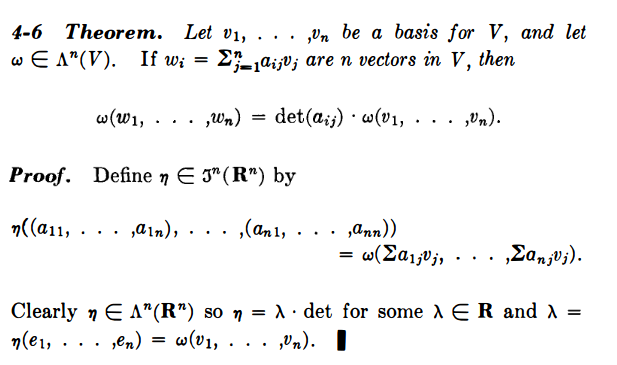
\includegraphics[width=\textwidth]{4.6.png}

{\color{def}Różniczka $dg\in\Gamma^1_0(\R^d)$} dla funkcji $g\in C^1(\R^d)$ to $1$-forma $dg={\partial g\over \partial x_1}dx^1+...+{\partial g\over \partial x_d}dx^d$. Dla funkcji różniczkowalnej $f:\R^d\to\R^m$ możemy też zdefiniować odwzorowanie liniowe $Df(p):\R^d\to\R^m$.

Jeśli mamy $k$-rozmaitość $M\subseteq\R^n$ i układ współrzędnych $f:W\to\R^n$ wokół $x=f(a)$. Ponieważ ranga $f'(a)$ wynosi $k$, to liniowe przekształcenie $f_*:T_a\R^d\to T_{f(a)}\R^m$ zadane wzorem
$$f_*((a,v))=(f(a), Df(a)(v)) <- \text{I CO ONO PONIEWAŻUJE???}$$
Wtedy $f_*(T_a\R^k)$ jest $k$-wymiarową podprzestrzenią $T_{f(a)}\R^n$. W dodatku jest to niezależne od wyboru układu współrzędnych, czyli jeśli $g$ też jest układem tam gdzie $f$ i $x=g(b)$, to 
$$g_*(T_b\R^k)=f_*(f^{-1}\circ g)_*(T_b\R^k)=f_*(T_a\R^k)$$
i to jest przestrzeń styczna $M$ w $x$, co Spivak oznacza $M_x$.
\smallskip

Kolejna funkcja, czyli 
$$f^*:\Gamma^k_0(\R^m)\to\Gamma_0^k(\R^d)$$
$$f^*(\omega)(a)(v_1,...,v_k)=\omega(f(a))(f_*(v_1),...,f_*(v_k))$$

\textbf{\large\color{acc}Twierdzenie}: istnieje jedyna $(p+1)$-forma $d\omega$ na rozmaitości $M$ taka, że dla każdego układu współrzędnych $f:W\to \R^n$ zachodzi
$$f^*(d\omega)=d(f^*\omega),$$
twierdzenie to jest bardzo podobne do zadania 3 z listy 22.

{\color{acc}Dowodzik:} Niech $f:W\to\R^n$ będzie układem współrzędnych takim, że $x=f(a)$ i niech $v_1,...,v_{p+1}\in M_x$. Wtedy istnieją unikalne $w_1,..,w_{{p+1}}\in\R^n$ takie, że $f_*(w_i)=v_i$. Zdefiniujmy 
$$d\omega(x)(v_1,...,v_{p+1})=d(f^*\omega)(a)(w_1,...,w_{p+1}).$$
Trzeba sprawdzić, że taka definicja $d\omega$ nie zależy od układu współrzędnych $f$ (patrz na uwagę wyżej, że $f_*(T_a\R^k)$ nie zależy od wyboru układu współrzędnych), więc $d\omega$ zostało dobrze dobrane. Co więcej, jasne jest, że $d\omega$ musiało zostać wybrane tak a nie inaczej, żeby śmigało.
\bigskip

Jeżeli $M$ jest $k$-wymiarową rozmaitością z brzegiem oraz $x\in \partial M$, wtedy $T_x\partial M$ jest $(k-1)$-wymiarową podprzestrzenią $k$-wymiarowej pole wektorowego $T_xM$. W $T_xM$ są dokładnie dwa wektory jednostkowe prostopadłe do $T_x\partial M$ i dokładnie jeden z nich może mieć ujemną wartość przez $f_*$, taki wektor nazywamy \emph{zewnętrznym wektorem normalnym} i oznaczamy $n(x)$. Definicja ta jest niezależna od wybranego układu współrzędnych. Tutaj warto wspomnieć, że jeśli rozmaitość na której pracujemy może mieć określoną orientację, która jest zachowywana przez różne układy współrzędnych, to ta orientacja determinuje też orientację na $T_x\partial M$ i nazywa się ją wtedy orientacją indukowaną.

\section{Wprowadzenie do twierdzenia Stokes'a}

Całkowanie $p$-formy $\omega$ po $p$-kostce singularnej $c$ definiujemy jako
$$\int_c\omega=\int_{[0,1]^p}c^*\omega$$
U nas kostka $c$ jest zgodna z układem współrzędnych $f$ opisanym na $W\supseteq[0,1]^p$. I tutaj znowu, jeżeli funkcjonujemy w obrębie rozmaitości orientowalnej i nasz układ współrzędny też jest orientowalny, to również $p$-kostka taka jest. W skrypcie chyba tak są kostki ogólnie zdefiniowane przy standardowym układzie współrzędnych.
\medskip

\textbf{\large\color{def}Twierdzenio-lemacik:} jeśli $f:\R^n\to\R^n$ jest różniczkowalna, to
$$f^*(hdx^1\land...\land dx^n)=(h\circ f)(det\;f')dx^1\land...\land dx^n$$
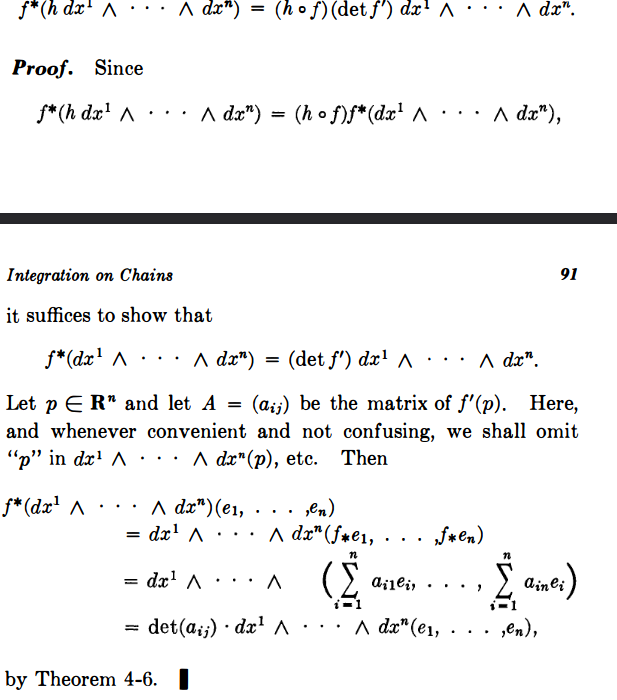
\includegraphics[width=\textwidth]{4.9.png}

\textbf{\large\color{acc}Twierdzenie:} dla dwóch orientowalnych $c_1,c_2:[0,1]^k\to M$ kostek zachowujących orientację w zorienotwanej $k$-rozmaitości $M$ oraz $k$-formy $\omega$ na niej, która zanika poza przekrojem tych kostek, mamy
$$\int_{c_1}\omega=\int_{c_2}\omega$$

{\color{acc}Dowodzik:} Z definicji wiemy, że
$$\int_{c_1}\omega=\int_{[0,1]^k}c^*\omega$$
Zauważmy, że $(c_2^{-1}\circ c_1)([0,1]^k)$ jest pewnym podzbiorem $[0,1]^k$, a ponieważ poza $c_1([0,1]^k)\cap c_2([0,1]^k)$, gdzie $c_2^{-1}\circ c_1$ zachowuje się jak identyczność, nasza forma się zeruje, to mamy
$$\int_{[0,1]^k}c^*\omega=\int_{[0,1]^k}(c_2^{-1}\circ c_1)^*c_2^*\omega.$$
Wystarczy teraz pokazać, że 
$$\int_{[0,1]^k}(c_2^{-1}\circ c_1)^*c_2^*\omega=\int_{[0,1]^k}c_2^*\omega.$$
Niech $g=c_2^{-1}\circ c_1$, a z kolei niech
$$c_2^*\omega=fdx^1\land...\land dx^k$$

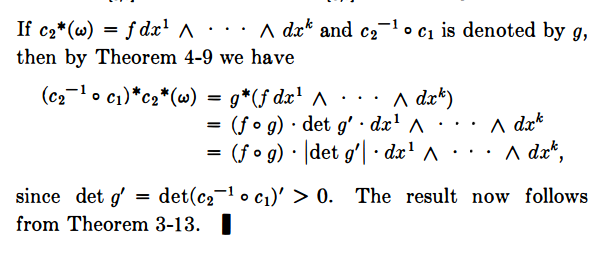
\includegraphics[width=\textwidth]{5.4.png}

I kończymy powołując się na:

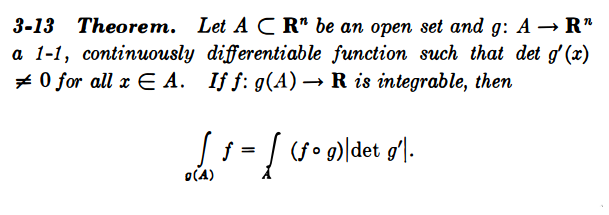
\includegraphics[width=\textwidth]{3.13.png}

Zgaduję, że orientacje były tutaj potrzebne, bo inaczej ten wyznacznik by nam się nie zgodził????

Jeżeli mamy rozmaitość $M$ i zdefiniowaną na nim $k$-formę $\omega$ oraz $k$-kostkę $c$ w $M$ taką, że poza $c([0,1]^k)$ $\omega$ się zeruje, to
$$\int_M\omega=\int_c\omega$$
i z powyższego twierdzenia wybór takiej kostki nie jest ważny, bo to wszystko to izomorfy będą.
\medskip

{\color{acc}I DALEJ TO JUŻ JEST STOKES, NA KTÓREGO ZA BARDZO MI MÓZG NIE DZIAŁA CHWILOWO}.


\bigskip

{\Large\color{acc}PYTANIA}:
\smallskip

Co oznacza grube $\mathbb{H}^k$ u Spivaka? Wiem, że otwarte podzbiory na których możemy opisywać układy współrzędnych w nim leżą.
\smallskip

Gdzie się w to wpisują kostki? To są takie podstawowe rozmaitości $k$-wymiarowe, a $I^(x)$ to ich układ współrzędnych? OK, BYŁY DALEJ XD
\smallskip

Czemu wystarczy przy $\color{red}\star\star\star$?

\end{document}